\chapter{Individual Cetacean ID via Automatic Most Likely Catalogue Matching}\label{ch:ID}

This Chapter examines the final component in the automatic photo-id pipeline, focussing on individual identification. The component takes as input photo-id catalogue images which have been passed through the dorsal fin detector and post-processing methodology outlined in Chapter \ref{ch:cetDet} to produce a list of most likely catalogue matches. It is important to note here that this component does not intend to replace photo-id researchers by performing the job for them. Instead, the component aims to vastly reduce the search space the researcher needs to examine in order to verify a catalogue match; the component suggests a list of most likely catalogue matches, but ultimately the final decision lies with the researcher.

Beginning by outlining the requirements an automatic system for most likely catalogue matching must meet, the Chapter then discusses possible approaches to the problem and justification for the selected approach. System development is discussed in detail, using the NDD AU SMRU dataset created in Chapter \ref{ch:NDD} for training and evaluation. Discussion of further processing techniques and their effect on most likely catalogue matching accuracy is discussed, alongside the current limitations of the approach. 

\section{Most Likely Catalogue Matching System Requirements}\label{ch:ID,sec:Requirements}

Before development can begin it is important to outline the requirements of a system capable of most likely catalogue matching. Unlike the detector which could be considered a coarse-grain task, identification of individual cetaceans is an extremely fine-grain problem as they are distinguished from each other using small prominent markings present on the dorsal fin. As the animals are free roaming, there can be high variation in how the fin is captured in the image, discussed in greater detail in Section \ref{ch:cetDet,sec:requirements,sub:environmental}. This can lead to photo-id catalogues with low inter-class but high intra-class differences between the individuals present, seen in Figure \ref{fig:segmented-ndd20-example}. As a result of this, any system capable of accurate catalogue matching must be able to recognise these minute differences between individuals even when there is high variation in the examples for each individual class. 

The system must also be capable of operating using all information provided to it. Other photo-id aides which perform most likely catalogue matching such as finFindR \cite{thompson_finfindr_2022} operate using only the trailing edge of the fin, with matching performed using notches and shape. This misses other prominent markings such as long term scarring or pigmentation, as well as the shape of other fin edges. As such, it may be the case that finFindR struggles when operating over a catalogue with few to no notches. To avoid this issue, the system developed must be capable of matching using all available prominent markings. 

Further, the system must also be capable of performing accurate catalogue matching under the presence of noise, both classified and misclassified. Datasets developed for the training of this system such as NDD AU SMRU contain a \texttt{noise} class which encapsulates all detected mask components which are erroneously retained after post-processing has been applied. This class has extremely high intra-class variance, however it is imperative the system is able to match erroneous components to it. Misclassified noise is defined as that which has been passed downstream as a result of being attached to a valid individual detection mask. In Figure \ref{fig:crop-with-unclassified-noise} for example, the swell captured in the post-processed crop would be considered misclassified noise. Any system performing automatic most likely catalogue matching must be resistant to small amounts of misclassified noise in order to produce accurate identity suggestions.

\begin{figure}
	\begin{center}
		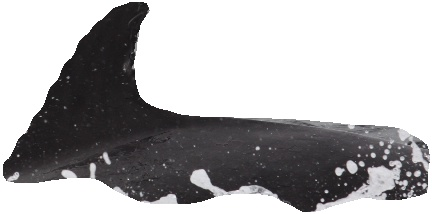
\includegraphics[scale=0.6]{Chapter5/figs/crop-with-unclassified-noise.jpg}
	\end{center}
	\caption{An example post-processed crop which contains some misclassified noise.}
	\label{fig:crop-with-unclassified-noise}
\end{figure}

Any developed system must also be capable of handling examples of individuals which are not present in the photo-id catalogue. Due to the free roaming nature of cetaceans (or indeed any wild animal) and the limitations on photo-id survey size dictated by both weather and workforce, there is no guarantee that every animal who makes use of the survey area will be captured. New animals may also become resident in the area through birth or migration. When these animals are eventually captured during a survey and their image processed, the system must be capable of recognising this as an individual not currently present in the catalogue and highlight this to the researcher. This is made more difficult given the extreme fine-grain nature of the catalogues. As a result, this requirement necessitates the system must be capable of recognising uncertainty or understand a notion of similarity between an input and the class examples present in the catalogue. 

In traditional computer vision classification models, if a new class were to be added this would require a large number of example images of the new class as well as model retraining or fine-tuning. However, cetacean researchers are highly unlikely to possess the technical skills required to retrain or fine-tune a computer vision model, and even if they do it is unlikely a large number of example images for the new individual would be available to do so. As such, the system must be adaptable enough so as to not require extensive retraining when new individuals are added to the catalogue.

\section{Possible Approaches}\label{ch:ID,sec:deciding}

Out of all requirements an automatic most likely catalogue matching system must meet, arguably the most important is the need for flagging of previously unseen individuals. As noted, this necessitates any underlying computer vision model to have some notion of uncertainty or similarity. It is this requirement that guided approach selection. 

\subsection{Bayesian Dropout}\label{ch:ID,sec:deciding,sub:bayesianDropout}

Traditional computer vision classification models do not meet this requirement. If an example image of a new individual was seen by a traditional CNN trained on a photo-id catalogue dataset, this model would still attempt to provide a classification based on the classes present at train time.  As deep computer vision models operate on point estimations of parameters, unlike Gaussian processes where the probability distribution is defined over a function, this removes the ability to produce helpful indicators of uncertainty such as prediction confidence bounds \cite{gal_uncertainty_2016}. 

One way to create a notion of uncertainty from this is through the use of Bayesian dropout. Vanilla dropout has found widespread use in the training of generalisable deep learning models. At train time, nodes in the model are intentionally not updated during a training step with some probability, usually defined as a hyperparameter with the goal of aiding model generalisability \cite{srivastava_dropout:_2014}. At test time, no dropout is performed and all nodes are utilised for the prediction. 

Bayesian dropout re-frames this technique by also performing dropout at test time, again with some hyperparameter defined probability \cite{gal_dropout_2016}. For each classification output, the model performs inference some large $N$ number of times. During each run model nodes are randomly disabled, zeroing out their weight and effecting the ability of the model to produce a prediction. By performing this multiple times and producing $N$ classifications, a probabilistic distribution is determined which can be used to understand the uncertainty of the model. A final overall prediction is generated by taking the mean of all $N$ predictions used to generate the probability distribution. If randomly dropping nodes at test time results in the model producing a wide variety of outputs, resulting in a diffused probability distribution, this suggests the model is uncertain; the lower the variance of the probability distribution, the more certain the model is. 

Whilst Bayesian dropout has found use in areas such as time-series forecasting \cite{laptev_time-series_2017}, widespread use has not been adopted in areas such as computer vision despite attempts \cite{kendall_what_2017}. This can be contributed to recognised issues such as ill-defined variational objective, the use of improper priors, and the potential for clarity issues between model uncertainty and risk \cite{hron_variational_2018, osband_risk_2016}. Further to this, the computational expense of performing Bayesian dropout is large given the need for multiple inferences required to produce the classification probability distribution.

This is the main reason why Bayesian dropout was not utilised for automated most likely catalogue matching. Should a researcher wish to process a large batch of images after a field survey for example, the need for multiple inferences would vastly inflate the time required for the batch operation to complete. Issues also arise meeting other system requirements. Even when using Bayesian dropout, the underlying model would still require retraining or fine-tuning to output newly catalogued individuals. 

\subsection{Siamese Neural Networks}\label{ch:ID,sec:deciding,sub:SNN}

Rather than producing a classification and measuring uncertainty as is the case with Bayesian dropout, Siamese Neural Networks (SNNs) aim to incorporate the notion of similarity into the model. This is achieved by connecting two or more identical CNNs in parallel, each sharing the same backbone architecture, initial and updated weights, and hyperparameters. Each CNN in the SNN is designed to produce an embedding, or a  $d$-dimensional representation, of the input. The size of this embedding is set via hyperparameter and dictates how many $d$ dimensions the output of the SNN will be. For example, if an SNN is created with an embedding size of 10, each CNN may take a high dimensional input of size \textit{width} * \textit{height} * \textit{channels} and output a 10-dimensional embedding, a float vector of size 10, which represents the input image. A visualisation of a two branch SNN can be seen in Figure \ref{fig:signet-SNN-architecture}.

\begin{figure}
	\begin{center}
		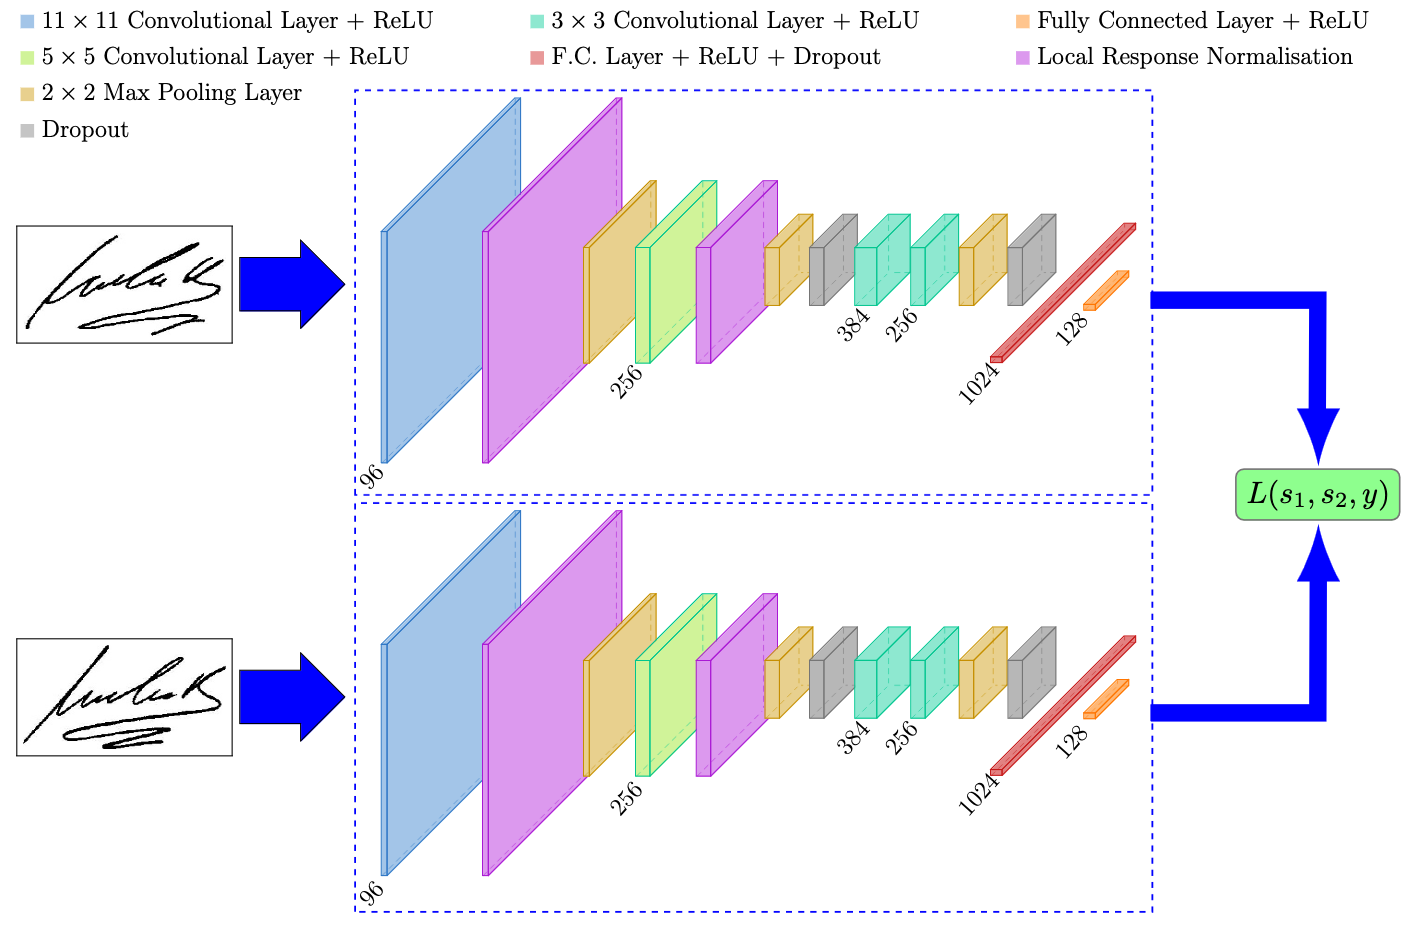
\includegraphics[scale=0.4]{Chapter5/figs/signet-SNN-architecture.png}
	\end{center}
	\caption{A visualisation of an example SNN architecture. Image from \cite{dey_signet_2017}.}
	\label{fig:signet-SNN-architecture}
\end{figure}

At train time, each CNN branch receives a different image and generates an embedding. These embeddings are compared to one another in order to optimise some loss function. By optimising in such a way that input images of the same class have similar embeddings but those of different classes are dissimilar, the SNN can be tuned to provide a measure of image similarity. Once trained only one branch of the model is retained. This allows a single image to be embedded by the model which can then be compared to the training examples.

It is this ability which has resulted in the wide use of SNNs for verification or identification problems in computer vision \cite{dey_signet_2017, wang_discriminative_2020}. Specifically in conservation tech, SNNs have found use in fine-grain species identification problems \cite{vetrova_hidden_2018, araujo_two-view_2022} as well as in more extreme fine-grain individual animal identification \cite{clapham_automated_2020}. 

\subsubsection{Clustering Embeddings in a Latent Space}\label{ch:ID,sec:deciding,sub:SNN,subsub:ClusteringEmbeddings}

By storing the embeddings generated for each trained class it is possible to produce a list of likely class predictions for a new image by measuring the Euclidean distance between the generated embedding and those previously produced when plotted into some $d$-dimensional latent space. If the SNN has trained in such a way as to produce low intra-class, high inter-class difference between generated embeddings then this will create class clusters when plotted in the latent space. 

An example of this behaviour can be seen in Figure \ref{fig:mnist-class-clusters-PCA} which shows a 2-dimensional visualisation, produced using Principle Component Analysis (PCA), of the embedding locations for a subset of the MNIST dataset \cite{lecun_gradient-based_1998}. Here, an SNN has been trained for 100 epochs to generate embeddings of images for the 10 unique classes. As can be seen, the model is able to generate embeddings in such as way as to cluster those of the same class in the latent space. Note that some clusters are visualised on top of each other due to the dimensionality reduction performed in order to show the latent space on the page. 

\begin{figure}
	\begin{center}
		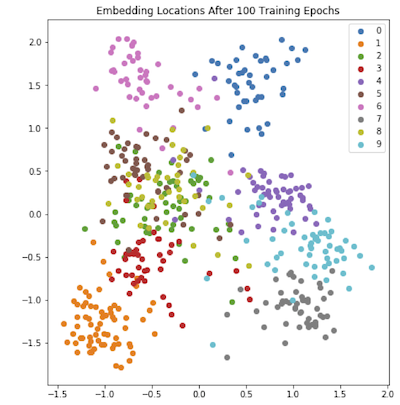
\includegraphics[scale=0.5]{Chapter5/figs/mnist-class-clusters-PCA.png}
	\end{center}
	\caption{A 2-dimensional visualisation of a multi-dimensional latent space produced by an SNN trained on the MNIST dataset \cite{lecun_gradient-based_1998} for 100 epochs.}
	\label{fig:mnist-class-clusters-PCA}
\end{figure}

It is important to note here that the value of the embeddings is not necessarily important, just the distances between them. Notice how all points in Figure \ref{fig:mnist-class-clusters-PCA} lie within approximately -1.5, 2.0 on the x-axis and -2.0, 2.0 on the y-axis. There is nothing inherently good or bad about an SNN that embeds within this range, all that matters is the points are clustering in their respective classes.

\subsubsection{Meeting the Outlined Requirements}\label{ch:ID,sec:deciding,sub:SNN,subsub:meetingOutlinedRequirements}
% Advantages and disadvantages for SNNs in relation to catalogue matching to show why the approach was taken.

When compared to Bayesian dropout, the computational expense of performing inference with an SNN is quite small. Whilst training requires the use of a branched CNN architecture in order to optimise the loss function, this is reduced to just one branch at inference time. Generating a list of most likely catalogue matches would only require an image to be passed through the network once in order to generate an embedding, and similarity via Euclidean distance measurement in the latent space is cheap to perform. As such, producing a list of most likely catalogue matches is overall more computationally efficient using SNNs as opposed to Bayesian dropout. 

The clustering of class embeddings in the latent space also allows for easy identification of potential previously unseen individuals. Passing the dorsal fin of an individual not present at train-time through the model would result in, theoretically, a distinct embedding which would plot into a unique point in the latent space far from any existing class clusters. By implementing a threshold on the Euclidean distance measurement, potentially unseen individuals could be easily flagged to the researcher for further investigation. Clustering also removes the need for re-training to allow for matching to previously unseen individuals when they are added to the catalogue. Adding a new class to the latent space can be achieved simply by defining embeddings to a new class cluster and including these in future distance measurements. 

In addition, SNNs are capable of operating over all information provided to them. This can be achieved by not limiting the embedding generation to one specific part of the dorsal fin. It also stands to reason that this embedding generation will be robust enough to deal with small amounts of retained background noise given a high enough number of dimensions. Overall, the use of SNNs for most likely catalogue matching far outweighs the use of Bayesian dropout. It is for this reason the decision was taken to first begin development of a model capable of most likely catalogue matching using SNNs.

\section{Siamese Neural Network Development}\label{ch:ID,sec:SNNDevelopment}
% Sec: Development of an SNN for Most Likely Catalogue Matching
% Discuss development of the SNN for catalogue matching using NDD AU SMRU
% Triplet Ranking loss, semi-hard triplet mining, prototypes from TDS blog
% Data augmentation, hyperparameter tuning

Before an SNN capable of most likely catalogue matching using the NDD AU SMRU dataset could be created, a development environment was first required to be selected. Initial testing first began using the Tensorflow framework \cite{abadi_tensorflow:_2016}, specifically version 1.14, as this would keep consistency with the dorsal fin detector developed in Chapter \ref{ch:cetDet}. 

Replication of the work undertaken by Vetrova \textit{et al.} \cite{vetrova_hidden_2018} for moth species identification proved promising. However, expanding to individual identification using the NDD AU SMRU dataset faltered when using Tensorflow, believed to be caused by a bug\footnote{Batch Normalisation Issues in Keras/Tensorflow: see \href{https://github.com/keras-team/keras/issues/11927}{github.com/keras-team/keras/issues/11927} and  \href{https://github.com/keras-team/keras/issues/9498}{github.com/keras-team/keras/issues/9498}} in how the Keras backend handles Batch Normalisation for models with multiple inputs resulting in model collapse, a phenomenon which results in the model returning the exact same output regardless of input. As a result of this, the decision was made to switch to using the PyTorch framework \cite{paszke_automatic_2017} which does not suffer these issues. 

\subsection{Pairwise vs Triplet Ranking Loss}\label{ch:ID,sec:SNNDevelopment,sub:lossFunction}

Training of any neural network is performed through the optimisation of a loss function. For SNNs, a group of loss functions known as Ranking Losses are utilised. Here, the goal is not to predict a class label but rather a distance between model inputs. As such, they are perfect for training SNNs. 

During training, an SNN will generate embeddings for some received inputs and generate a similarity value (e.g. via Euclidean distance when plotted into a latent space). This similarity value is then used to optimise the Ranking Loss, which in turn tells the model how to adjust to create better embeddings, for example how to bring two embeddings closer when they are of the same class. The type of Ranking Loss utilised for training and the number of branches present in the SNN are intertwined. Two of the most commonly used Ranking Losses are Pairwise Ranking Loss and Triplet Ranking Loss.

\subsubsection{Pairwise Ranking Loss}\label{ch:ID,sec:SNNDevelopment,sub:lossFunction,subsub:Pairwise}

SNNs which make use of two branches can be optimised using a Pairwise Ranking Loss, a visualisation of which can be seen in Figure \ref{fig:pairwise_ranking_loss_faces}. Here the model is trained using data points made up of two inputs. The first input is called the Anchor, an input which defines the class the model is training to optimise for. The second input can be either a Positive containing another example of the Anchor class, or a Negative containing an example input of some class other than the Anchor. 

\begin{figure}[h]
	\begin{center}
		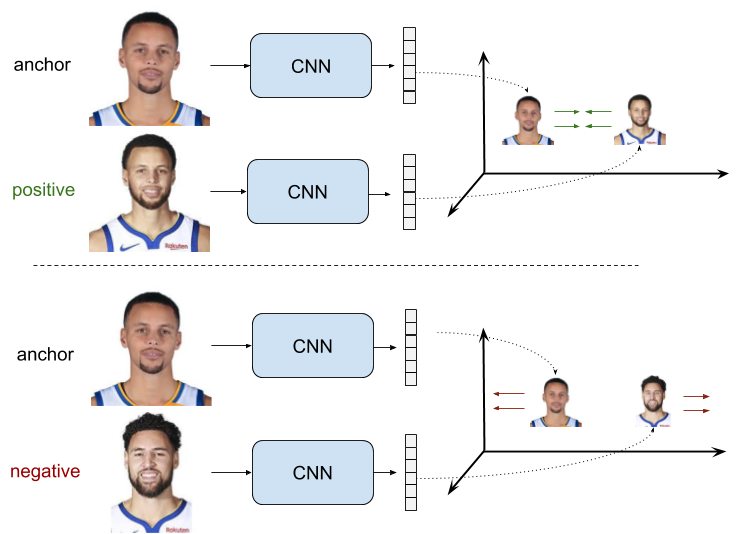
\includegraphics[scale=0.4]{Chapter5/figs/pairwise_ranking_loss_faces.png}
	\end{center}
	\caption{A visualisation of SNN optimisation using Pairwise Ranking Loss. Image from \cite{gomez_understanding_2019}.}
	\label{fig:pairwise_ranking_loss_faces}
\end{figure}

Using these two input types Pairwise Ranking Loss can be used to optimise in such a way that the model learns to produce embeddings with a small distance between Anchors and Positives, and a large distance between Anchors and Negatives. Mathematically Pairwise Ranking Loss can be defined as such:

\begin{equation}
	L =
		\begin{cases}
			D(A,P) & \text{if Positive Pair}\\
			max(0, m - D(A,N)) & \text{if Negative Pair}\\
		\end{cases}       
\end{equation}

Where $L$ is the loss, $D(A,P)$ is the distance between the Anchor and the Positive, and $D(A,N)$ is the distance between the Anchor and the Negative. When optimising for Positive Pairs the loss function will only ever return 0 when the distance between the Anchor and the Positive is 0, ensuring these embeddings are nearly always pulled closer. When optimising for Negative Pairs, the loss function will return 0 when the distance between the Anchor and the Negative is greater than some margin $m$. As such, a weight update is not performed when the distance between the Anchor and the Negative is sufficiently large.

% Problem with Pairwise: Positive Pair optimisation eventually leads to collapse whereby examples of the same class produce exactly the embedding, negativley effecting the model's ability to understand similarity and input variation. 


% Sec: SNN Evaluation
% Finding the best model, top-n accuracy explanation
% Unseen inidividual thresholding using prototypes and KNN
% Limitations (unseen individuals may just be changed - at least we're flagging and having a human decide. re-training needed for each catalogue.)

% Sec: Effect of Input Image Variation
% Black and white
% Two classes for each side of the fin (seems to work but inconclusive given size of dataset)

% Sec (Ch if above ~20pages+?): Full Pipeline Evaluation
% WMMC dataset discussion
% Go through the pipeline, highlighting each step
% Show SNN approach is generalisable with retraining, Mask-RCNN does not need re-training
% Hyperparam tuning SNN here helps but only slightly (near optimal hyperparams found for the problem space?)

% Sec: Conclusion
% Summary of the work
% Produced a model capable of meeting requirements
% State we have extended the literature in use of image embeddings and latent space distance measurements for conservation (vetrova etc) and individual re-id (bearID)



  


%%%%%%%%%%%%%%%%%%%
